\documentclass{ZJUthesis}
\hypersetup{colorlinks=false}
\begin{document}
%%%%%%%%%%%%%%%%%%%%%%%%%%%%%
%% 正文字体设定
%%%%%%%%%%%%%%%%%%%%%%%%%%%%%
\fangsong

%%%%%%%%%%%%%%%%%%%%%%%%%%%%%
%% 论文封面部分
%%%%%%%%%%%%%%%%%%%%%%%%%%%%%
\classification{TN292.11}
\serialnumber{10335}
\PersonalID{10930020}

\title{量子阱混杂技术以及}
\titletl{其在光子集成回路中的应用}

\Etitle{Quantum Well Intermixing Technology and}
\Etitletl{its Application in Photonic Integration Circuits}

\author{张欣}
\degree{博士}

\supervisor{何建军}
\major{光电系}
\researchdm{光通信技术}
\institute{光电系}

\submitdate{2015年5月20日}
\defenddate{2015年6月20日}

\makeCoverPage

%%%%%%%%%%%%%%%%%%%%%%%%%%%%%%
%% 中文题名页内容
%%%%%%%%%%%%%%%%%%%%%%%%%%%%%%
\reviewersA{}
\reviewersB{}
\reviewersC{}
\reviewersD{}
\reviewersE{}

\chairman{}
\commissionerA{}
\commissionerB{}
\commissionerC{}
\commissionerD{}
\commissionerE{}

\maketitle
%%%%%%%%%%%%%%%%%%%%%%%%%%%%%%
%% 英文封面内容,硕士论文可不要此页
%%%%%%%%%%%%%%%%%%%%%%%%%%%%%%
\englishtitle{Quantum Well Intermixing Technology and}
\englishtitletl{its Application in Photonic Integration Circuits}

\EreviewersA{}
\EreviewersB{}
\EreviewersC{}
\EreviewersD{}
\EreviewersE{}

\Echairman{}
\EcommissionerA{}
\EcommissionerB{}
\EcommissionerC{}
\EcommissionerD{}
\EcommissionerE{}

\makeenglishtitle
%%%%%%%%%%%%%%%%%%%%%%%%%%%%%%
%% 原创声明与版权协议页
%%%%%%%%%%%%%%%%%%%%%%%%%%%%%%
\makeOSandCPRTpage

%%%%%%%%%%%%%%%%%%%%%%%%%%%%%%
%% 论文部分开始
%%%%%%%%%%%%%%%%%%%%%%%%%%%%%%
\ZJUfrontmatter

%%%%%%%%%%%%%%%%%%%%%%%%%%%%%%
%% 致谢页
%%%%%%%%%%%%%%%%%%%%%%%%%%%%%%
\begin{thanks}
在即将完成学业的时候,想起自己在求是园度过的九年时光,我百感交集。人的一生说来很短暂,而青春的岁月更是屈指可数。我将生命中最美好的时光献给这里,我无怨无悔。同时,我也心存感激,感谢身边所有的人,陪我度过这人生中最美好的时光。

首先,我感谢我的父母。看着身边的孩子早早的工作,成家,甚至有了自己的孩子,我想你们的等待似乎太满长了一些。辛苦劳动了一辈子,现在终于可以等到享福的时候了。爸爸妈妈,你们为我骄傲,我为你们骄傲。

然后,我感谢我的导师何建军教授。何老师渊博的学识、严谨的态度让我终生难忘,
他精益求精、一丝不苟的工作作风让我敬佩不已。非常感谢何老师科研上的精心栽培和
生活上的热心关怀。

同时,我感谢实验室所有成员对我工作的大力支持和帮助。感谢彭盛华硕士带领我进入课题,给予我学术上的启蒙性的指导和建议。感谢李明宇博士、王磊博士、刘德坤博士、金嘉亮博士、金磊博士、马骁博士、朱宏力、邹立对我的关怀和照顾。感谢庄园、孟剑俊、邓浩瑜在学术上的大力支持,让我明白了什么叫做后生可畏。感谢紫金港东五的时尧成博士、胡师傅、陈辉对我实验的大力帮助。这一切都会成为我一生美好而难忘的回忆。

最后,我要感谢为我辛苦服务了六年的超净室设备和教三测试平台,特别是牛津ICP、快速退火炉、通光测试台、PL 测试系统。在我的眼力,你们一直是有生命的存在。
\end{thanks}

%%%%%%%%%%%%%%%%%%%%%%%%%%%%%%
%% 摘要
%%%%%%%%%%%%%%%%%%%%%%%%%%%%%%
\begin{abstract}
如电信业进入二十一世纪对带宽的需求持续增加。需要大量带宽的应用不断被开发和引入,将很快被重载光纤网络。的波分复用(WDM)的出现,极大地增加了每个光纤内传送的数据量,但增加了系统维护的成本。几个关键技术都有望彻底改变通信产业。的广泛可调谐激光器,有能力调整到国际电信同盟(ITU)网格上的任何频道的推出将极大地通过不遗余力的功能,使系统运营商降低库存的激光,可调谐取代固定波长激光器降低系统维护成本激光器。采用可调谐激光器的下一代网络应用正在探索增加系统的功能。另一项关键技术,光子集成电路(PIC),将允许通过单片集成降低成本。除了降低成本的简单问题来的高功能设备,允许一个更大的利用系统资源,并基于这些设备的新网络架构的发展的可能性。这项工作涉及到这两个技术进步的耦合创造的波长敏捷的PIC的新品种。这些设备是新一代,高效率,高带宽的光纤网络发展的理想构建模块。一种基于量子阱混合(QWI)新型加工技术,专门为这个目的而开发的。该QWI过程允许的多重量子阱带边,最好是一特定于每个集成部件的形成。这个过程施加到V-耦合腔激光器(VCCL)与提高器件特性的目的。过程中的波长敏捷的PIC制造的适用性是通过电吸收调制器具有一个独特的量子阱带边的单片集成证实。集成的器件的输出功率,调谐范围,边模抑制比,消光,和带宽方面表现出优异的性能。

\keywords{光子集成回路,量子阱,量子阱混杂,半导体激光器}
\end{abstract}

%%%%%%%%%%%%%%%%%%%%%%%%%%%%%%
%% 英文摘要
%%%%%%%%%%%%%%%%%%%%%%%%%%%%%%
\begin{englishabstract}
As the telecommunications industry enters the twenty-first century the demand for bandwidth continues to increase. Applications requiring vast amounts of bandwidth continue to be developed and introduced into a fiber optic network that will soon be overloaded. The advent of wavelength division multiplexing (WDM) has greatly increased the quantity of data transported within each optical fiber, yet increased the cost of system upkeep. Several key technologies are poised to revolutionize the communications industry. The introduction of widely-tunable lasers that are capable of tuning to any channel on the international telecommunications union (ITU) grid will dramatically reduce the cost of system upkeep through sparing functions, allowing system operators to reduce laser inventory, replacing fixed wavelength lasers with tunable lasers. Next generation networking applications using tunable lasers are being explored for increasing the functionality of the system. Another key technology, the photonic integrated circuit (PIC), will allow for cost reduction through monolithic integration. Beyond simple issues of cost reduction come the possibility of high functionality devices allowing a far greater use of system resources and the development of new network architectures based on these devices. This work involves the coupling of these two technological advancements to create a new breed of wavelength agile PICs. These devices are the ideal building blocks for the development of next generation, efficient, high bandwidth fiber optic networks. A novel processing technique based on quantum well intermixing (QWI) was developed specifically for this purpose. The QWI process allows for the formation of multiple quantum well band edges, ideally one specific to each integrated component. The process was applied to V-coupled cavity laser (VCCL) with the goal of improving device characteristics. The applicability of the process to the fabrication of wavelength agile PICs is demonstrated through the monolithic integration of electro-absorption modulators possessing a unique quantum well band edge. The integrated devices exhibited excellent characteristics in terms of output power, tuning range, side mode suppression ratio, extinction, and bandwidth.

\englishkeywords{photonic integrated circuit, quantum well, quantum well intermixing, semiconductor laser}
\end{englishabstract}

%%%%%%%%%%%%%%%%%%%%%%%%%%%%%%
%% 目录页
%%%%%%%%%%%%%%%%%%%%%%%%%%%%%%
\ZJUcontents

%%%%%%%%%%%%%%%%%%%%%%%%%%%%%%
%% 正文内容部分开始
%%%%%%%%%%%%%%%%%%%%%%%%%%%%%%
\ZJUmainmatter

\chapter{绪论}

随着时代的进步,光通信技术作为引领人类信息革命的关键技术,正在蓬勃和飞速的发展。而光通信的芯片制造技术,又是光通信技术中门槛最高,附加值最大的技术,也是整个光通信领域最核心的技术。可以说,谁掌握了芯片制造的前沿技术,谁就站在了光通信技术的制高点上。近年来,单片集成和大范围可调谐激光器,正在逐渐被人们所重视,并成为了芯片制造的前沿技术。在接下来的内容中,单片集成和大范围可调谐激光器这两项技术将被详细讨论。

\section{单片集成}

在光通信行业,为了带来革命性的高功能、低成本的设备,单片集成是一项关键技术。芯片上的光的产生、检测、运输,由过去分立器件实现,到单片集成器件实现,是一个重大进步。这不仅将整体的成本拉了下来,还会导致新一代的高功能的集成光子回路(PIC)芯片的产生。

单片集成技术事实上已经在电子工业中广泛应用起来。现在的电子集成电路(IC),可以把成千上万个晶体管、电阻、电容等器件,集成在同一块芯片上。集成电路的出现,不仅相对于分立器件来说降低了成本,最重要的是,这导致了一系列高功能的集成电路的产生。光通信领域也面临着类似的转变。

目前,光通信领域中的大多数光电元器件依然是离散工作的。也就是说,每个器件是被设计用来执行一个特定的任务的。几个具有不同功能的器件互相连接,最终实现预定的效果。这种方法有一个优点,即每个器件的特定功能都进行了优化,使得整个设备可以完美地完成任务。但是,用这种连接的方法也有一些缺点。一个缺点是每个离散芯片之间的光耦合的开与关。在器件之间使用模式转换器,是半导体芯片减少耦合损耗的显著进展,但它仍然是光损耗的一个主要来源。另一个缺点是每个离散器件的封装成本,也是光电器件成本的重要来源。

将光电器件单片集成在同一块芯片上,不仅可以彻底解决耦合的问题,还可以减少封装成本。然而,其缺点是,每个器件必须制作在同一块芯片上,这样做在技术上是很困难的。过去已经有几种技术被用于单片集成,例如对接再生(BJR),以及选择性区域外延(SAG)。

在单片集成光电元器件时,有一些必须满足的要求。首先,每一个集成组件必须实现预期的功能。每一个组件也许不需要像分立器件那样性能好,但是至少也需要达到集成在一起实现整体功能的基本要求。第二个要求是一个组件的操作不会产生不利于另一个器件的影响。每一个组件在一个集成回路中,应当与其他的部件在功能上分离,就好像它是一个分立器件。

在实现单片集成的方法中,也有一些一般性的指引。首先,所使用的方法不应该是费时或昂贵的。这是对现有的分立器件实现降低成本的关键。其次,集成不应该导致整体性能下降。这是一个困难的任务,因为每个分立器件在设计时都是独立优化的。然而,如前所述,集成组件必须能实现特定功能,但并不一定需要分立器件的性能互相匹配。这提供了一定的灵活性,即可能允许使用相同的生长和加工平台去制造具有不同功能的设备。最后,该过程的复杂性,在集成元件数目增加时应保持不变。不然,制造过程可能会增加制造成本,并可能导致成品率降低。接下来我们将回顾一些过去使用的单片集成方法。

已经有一些很好的方法用来生产简单的光子集成回路了。这样的方法包括但不限于对接再生长 \cite{binsma1997characterization-BJR},选择性区域生长 \cite{aoki1993ingaas-SAG},和使用偏置量子阱 \cite{mason1999widely-offset}。 首先,对接再生长就是把一部分的波导芯层去掉,再用另一种材料再生长。这个过程中,要精确地刻蚀原来的波导的芯层,然后重新生长的波导材料又要在成分和厚度上与原来的匹配,这是非常困难的。另一种SAG方法的关键是掩模的选择性生长。在这个过程中,在外延之前需要先在表面生长一层掩模。掩模的形状可以决定外延生长的组分和厚度。在晶片的某些能带边缘,这种方法是有用的,但是在这些区域内由于厚度的变化,光学限制因子就不能被单独优化了。最后,偏置量子阱就是在波导之上的一层量子阱被选择性地除去。这种方法已经成功地被用来制造各种集成芯片 \cite{mason1999widely-offset} \cite{mason2000design-offset} \cite{mason1998tunable-offset} \cite{fish1998compact-offset}。 然而,使用偏置量子阱时,整块芯片只能使用一到两个能带边缘,对于制造复杂的光子集成回路就束手无策了。

在生产简单的光子集成回路时,一般只有少于三个的能带边缘,这些方法能很好地工作。但对于较大规模的集成就不适合了。大规模的集成需要多个能带边缘,理想情况下每个集成组件一个。例如,半导体激光器为了让增益峰和工作波长一致,就需要一个能带边缘,而电吸收调制器需要的能带要比激光器的能带稍微大一些。如此一来,首先确定了每个器件的能带之后,再来对各个器件的性能进行优化。

\section{大范围可调谐激光器}

随着密集波分复用(DWDM)技术的广泛使用,波长敏捷型光子集成回路变得越来越重要。波分复用技术通过在一路光纤中传输多路光信号的方法,增加了网络的带宽。国际通信联盟(ICU)制定了WDM的基本规则。现在的光信道的间隔为100GHz或0.8纳米,未来将会变成50GHz或25GHz。要实现WDM,就需要激光器覆盖ICU规定的每个信道。想要覆盖这么多的信道,使用大范围可调谐激光器是一个明智的选择。

现在人们在实验室已经制造出了很多种大范围可调谐激光器。其中一种就是V型腔激光器。V型腔激光器的示意图如图\ref{fig_vccl}所示。其主要部分包含两个长度不同的光学谐振腔,一个耦合相位为 180°的半波耦合器以及一个波长调谐区。另外在V字型的闭合端(图\ref{fig_vccl}中右端)有一个耦合器,V字型的开口端(图\ref{fig_vccl} 中左端)为一个多模耦合器(MMI)。

\begin{figure}[htb]
  \centering
  
\includegraphics[width=0.7\textwidth]{./Pictures/vccl.eps}\\
  \caption{V型腔激光器的光学显微镜图\cite{jin201116-VCCL}}\label{fig_vccl}
\end{figure}

其中第一个光学谐振腔由一段光波导以及两端的深刻蚀反射槽构成,该段光学波导上面镀有一段电极用来注入电流以提供激光器谐振所需的增益,我们称之为固定增益腔(Fix Gain Cavity)。第二个光学谐振腔由两段光学波导以及两端的深刻蚀反射槽构成,其中一段波导提供增益,另一段波导为无源波导,可以通过注入电流来改变其光学长度从而来调谐激光器的工作波长,因此称之为信道选择腔(Channel Selector Cavity)。两段波导中间由一个浅刻蚀槽隔开。在V字型的闭合端,两个谐振腔中间由一个耦合相位为 180°的半波耦合器相连,通过设计优化两个腔之间的耦合系数可以使得整个复合耦合腔激光器实现高的边模抑制比和良好的单模特性。另外波长调谐区离耦合区较远,使得其折射率的改
变几乎不影响两个谐振腔之间的耦合系数。左端的MMI 耦合器用来将两根波导的输出光耦合到一跟波导,同时可以通过调节一个臂的注入电流来切换光输出的端口,用以做空间光开光。

为了实现激光器工作波长的数字式调谐,固定增益腔的长度要根据激光器的工作波长来确定,使得固定增益腔的谐振频率的间隔与预先要求的频率间隔一致,例如根据ITU的规定,各个通信波长的间隔为200GHz、100GHz或者50GHz等。谐振腔的频率间隔可由下式确定:

\begin{equation}
  \Delta f = \frac{c}{2 n_g L}
\end{equation}

其中$c$是真空中的光速,$n_g$是波导的有效群折射率,$L$是固定增益腔的长度。

同样,第二个谐振腔(信道选择腔)的频率间隔$\Delta f ^\prime$由式\ref{eqa_Daltafprime}决定:
\begin{equation}\label{eqa_Daltafprime}
  \Delta f ^\prime= \frac{c}{2 n_g^\prime L^\prime} = \frac{c}{2 (n_a L_a + n_b L_b)}
\end{equation}

其中$L_a$和$L_b$分别为信道选择腔的增益区以及波长调谐区的长度,同样$n_a$和$n_b$分别为信道选择腔的增益区以及波长调谐区的有效群折射率。$L^\prime=L_a+L_b$是信道选择腔的总长度,$n_g^\prime=(n_a L_a + n_b L_b)/L^\prime$是信道选择腔的平均有效群折射率。

信道选择腔的频率间隔$\Delta f ^\prime$选择为与固定增益腔的频率间隔$\Delta f$有一个微小的差别,这使得在工作物质的增益窗口内,两者只有一个谐振峰恰好重合(如图\ref{fig_Deltaf}所示)。两个谐振腔相邻的互相重合的谐振峰之间的间隔为组合腔的自由光谱范围(FSR),其大小由式\ref{eqa_Daltafc}决定。为了避免两个波长同时被激发,$\Delta f_c$一般来讲必须大于激光器工作物质增益窗口的宽度。
\begin{equation}\label{eqa_Daltafc}
  \Delta f_c = \frac{\Delta f \Delta f^\prime}{|\Delta f-\Delta f^\prime|}
\end{equation}
\begin{figure}[htb]
  \centering
  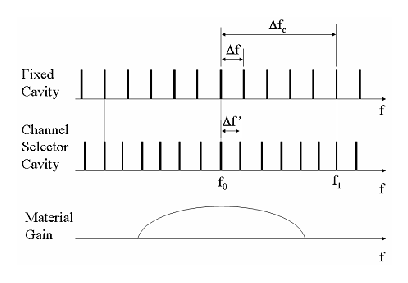
\includegraphics[width=0.7\textwidth]{./Pictures/deltaf.eps}\\
  \caption{固定增益腔和信道选择腔的谐振频率位置关系的示意图,以及激光工作物质的增益光谱曲线}\label{fig_Deltaf}
\end{figure}

固定增益腔以及信道选择腔的谐振频率分别为:
\begin{equation}
  f = \frac{mc}{2nL}
\end{equation}
\begin{equation}
  f^\prime = \frac{m^\prime c}{2n^\prime L^\prime}
\end{equation}
其中$m$和$m^\prime$都是整数,$n$和$n^\prime$分别为两个腔的平均有效折射率,$L$和$L^\prime$ 分别为两个腔的长度。信道选择腔的谐振频率$f^\prime$可以通过改变波长调谐区的折射率$n_b$从而改变整个腔的有效折射率$n^\prime$而改变。频率调谐量由下式决定:
\begin{equation}
  \frac{\delta f^\prime}{f^\prime} = -\frac{\delta n^\prime}{n^\prime}=-\frac{\delta n_b L_b}{n_b L^\prime}
\end{equation}

由于激光器的工作频率为固定增益腔与信道选择腔谐振峰重合的频率,因此$|\Delta f-\Delta f^\prime|$一个较小的变化将会导致激光器工作频率跳变一个信道。因此,激光器工作频率的改变量被放大了一个因子$\Delta f/|\Delta f-\Delta f^\prime|$,即:
\begin{equation}
  \delta f = \frac{\Delta f}{|\Delta f-\Delta f^\prime|} \delta f^\prime
\end{equation}

这种效应称作为游标效应。取样光栅(Sample Grating ,SG) 、超结构光栅(Super Structure Grating,SSG)也是利用类似的原理,但是取样光栅,超结构光栅的频率间隔是由光栅的调制周期决定,而且通常至少需要10个周期以上,为了获得同样的频率间隔,取样光栅超结构光栅的器件长度通常为V 型腔的20倍左右。

鉴于通常的ITU 标,假设$\Delta f=100GHz$,$\Delta f^\prime=90GHz$,则激光器工作频率的调节范围与仅靠调节折射率相比扩大了10倍。在上述数据下,设波导的有效群折射率为3.215,则固定增益腔以及信道选择腔的长度分别为:$L=466.24\mu m$,$L^\prime=518.31\mu m$,其长度与传统的DFB以及法布里- 珀罗激光器相当。相比之下,取样光栅、超结构光栅DBR激光器,由于受到器件长度以及损耗的限制,通常的信道间隔至少为600GHz,而对于通常的密集波分复用系统(DWDM)信道间隔一般为50GHz~200GHz,很难实现完全的数字式调谐。对于V型耦合腔宽带可调谐激光器,则完全不受此限制,并且利用深刻蚀槽做反射面技术,通过全息平版照相(photolithographic)技术可以精确控制激光器谐振腔的长度。激光器工作波长与ITU标准的些许偏离可以由微调固定腔的注入电流以及温度调谐来补偿。

\section{本文概述}

本文的主要工作就是改进V型腔激光器的调谐功能。将以往基于温度变化的波长调谐技术,转变成基于载流子注入的波长调谐技术。所使用到的关键技术就是氟化氪紫外激光器诱导的量子阱混杂技术。本文第二章将介绍量子阱混杂技术以及从理论上解释其原理。第三章将介绍氟化氪紫外激光器诱导的量子阱混杂技术的工艺步骤和实验结果。第四章将介绍该技术用于V型腔激光器之后的效果。第五章进行总结与展望。

%%%%%%%%%%%%%%%%%%%%%%
\chapter{单片集成技术概述}

\section{BJR}

\section{SAG}

\section{offset QW}

\section{Si-III/混合集成}

\section{量子阱混杂技术}

%%%%%%%%%%%%%%%%%%%%%%%%%%%%%%%%%%%
\chapter{量子阱混杂技术回顾与理论模拟}

本章首先回顾了各种量子阱混杂技术,并比较他们的优缺点。然后从理论上介绍了量子阱混杂的机理,利用量子阱能带理论和经典的扩散方程,模拟了磷化铟量子阱能带移动的现象。

\section{量子阱混杂技术回顾}

量子阱混杂是一个量子阱的阱和势垒相互扩散的过程。在这个过程中,随着扩散的不断增强,量子阱的形状和厚度也随之不断变化,从而导致能带的变化。变化之后的能带对应的能量一般来说都是增加的,也就是波长发生蓝移。在一般情况下,量子阱的阱和势垒之间的界面是亚稳态的,在一定的条件下,例如高温下,量子阱的阱和势垒的原子会相互扩散。量子阱混杂的目标不是简单地使阱和势垒相互扩散,而是在整个区域中做选择性的扩散。

已经有很多种方法可以实现量子阱混杂的效果,例如杂质诱导无序(IID) \cite{holonyak1998impurity-IID} ,无杂质空位增强无序(IFVD) \cite{si1998area-IFVD},光吸收诱导无序(PAID) \cite{mckee1997monolithic-PAID},离子注入增强扩散\cite{charbonneau1998photonic-implantation}等等。

%%%%%%%%%%%%%%%%%
\chapter{量子阱混杂技术的理论模拟}

\section{量子阱原理}

\section{量子阱计算}

\section{混杂模型}

\section{混杂前后的禁带宽度对比}

%%%%%%%%%%%%%%%%%%%%%%
\chapter{量子阱混杂技术的工艺研究}

\section{氩气等离子体轰击法}

\section{KrF准分子激光器照射法}

%%%%%%%%%%%%%%%%%%%%%%

\chapter{量子阱混杂技术在集成光子回路中的应用}

\section{包含量子阱混杂技术的V型腔激光器的设计}

\section{包含量子阱混杂技术的V型腔激光器的制作过程}

\section{测试结果}

\section{结果分析}

%%%%%%%%%%%%%%%%%%%%
\chapter{总结和展望}

\section{本文总结}

\section{本文展望}

\ZJUbackmatter
%%%%%%%%%%%%%%%%%%%%%%%%%%%%%%
%% 参考文献
%%%%%%%%%%%%%%%%%%%%%%%%%%%%%%
\bibliographystyle{unsrt} %% plain.bst
\bibliography{thesisbib} %% thesisbib.bib

%%%%%%%%%%%%%%%%%%%%%%%%%%%%%%
%% 个人简历
%%%%%%%%%%%%%%%%%%%%%%%%%%%%%%
\begin{resume}
\begin{enumerate}
\item{1986年10月12日,出生于浙江省杭州市}
\item{2009年6月,在浙江大学信息工程光电系获得工学学士学位}
\item{2014年6月,在浙江大学光电系获得工学博士学位}
\end{enumerate}
\end{resume}

%%%%%%%%%%%%%%%%%%%%%%%%%%%%%%
%% 发表论文目录
%%%%%%%%%%%%%%%%%%%%%%%%%%%%%%
\begin{publications}
\begin{enumerate}
\item{Yuan Zhuang, \textbf{Xin Zhang}, Mohammad Kaleem and Jian-Jun He. "Large bandgap shift by UV excimer laser induced quantum well intermixing for photonic integration." Asia Communications and Photonics Conference and Exhibition. Optical Society of America, 2013.}
\item{Kaleem, Mohammad, et al. "UV laser induced selective-area bandgap engineering for fabrication of InGaAsP/InP laser devices." Optics and Laser Technology 51 (2013): 36-42.}
\item{Kaleem, Mohammad, \textbf{Xin Zhang}, and Jian-Jun He. "Bandgap engineering of InGaAsP/InP laser structure by argon plasma induced point defects." Communications and Photonics Conference (ACP), 2012 Asia. IEEE, 2012.}
\item{彭盛华, \textbf{张欣}, and 何建军. "氩等离子体诱导量子阱混合技术." 浙江大学学报 (工学版) 6 (2011): 015.}
\item{\textbf{Zhang, Xin}, and Jian-Jun He. "Optical loss of bandgap shifted InGaAsP/InP waveguide using argon plasma-enhanced quantum well intermixing." Advances in Optoelectronics and Micro/Nano-Optics (AOM), 2010 OSA-IEEE-COS. IEEE, 2010.}
\item{Shenghua Peng, \textbf{Xin Zhang} and Jian-Jun He. "Nitrogen plasma enhanced quantum well intermixing in InGaAsP/InP laser structure." Asia Communications and Photonics Conference and Exhibition. Optical Society of America, 2009.}
\item{何建军, \textbf{张欣}, 彭盛华. "一种量子阱混合方法." 中国发明专利CN101697341A}
\item{何建军, \textbf{张欣}, 彭盛华. "一种量子阱混杂方法." 中国发明专利CN101774540A}
\end{enumerate}
\end{publications}

\end{document}
